\chapter{Results}\label{ch:results}

This chapter will provide various numerical test results of SF-PIF methods.
In order to examine the numerical capabilities of the SF method,
several well-known numerical benchmark problems are conducted,
and the traditional SSP-RK methods' results will be provided with the same initial conditions
as counterparts of SF-PIF methods for comparisons.
SF-PIF3 and SF-PIF4 will refer to the \textit{recursive} SF method in~\cref{sec:recursive_sf}
with third-order and fourth-order PIF methods, respectively,
and RK3 and RK4 will refer to the three-stage, third-order SSP-RK method~\cref{eq:ssp_rk3},
five-stage, fourth-order SSP-RK method~\cref{eq:ssp_rk4}, respectively.
The original SF approach (\cref{sec:original_sf}) with the PIF method is denoted by oSF-PIF\@.
The conventional five-point central differencing formulae~\cref{eq:pif_central_dfdx,eq:pif_central_dfdxx,eq:pif_central_dfdxy}
are used for SF-PIF and PIF methods otherwise specified.

\section{Performance of SF-PIF method}\label{sec:result_performance}
The main advantage of the PIF method is the performance gain compared to the SSP-RK methods.
This section will compare the performance of PIF methods (with or without the SF approach)
and the SSP-RK method. The main purpose of this section is to check if the SF-PIF methods provide
improved performance while maintaining the same accuracy as SSP-RK methods.
Theoretically speaking, the SF and oSF approach should not affect the solution's accuracy and stability,
so the original PIF method's results are presented for comparisons.

All test results in this section use the standard fifth-order WENO-JS method (\cref{subsec:weno})
for the spatially high-order reconstruction scheme.
Therefore, the expected truncation error is \( \mathcal{O}(\Delta s^{5}, \dt^{q}) \),
where \( q \) is the order of the temporal scheme.

\subsection{Sine wave advection}

The first choice of the benchmark problem is the sine wave advection
to test if the desired solution accuracy is retrieved in smooth flows.
The initial condition follows the setup in~\cite{lee2017piecewise},
where the density profile is initialized with a sinusoidal wave,
\( \rho (x) = 1.5 - 0.5\sin(2\pi x)\).
The $x$-velocity and
the pressure are set as constant values of \( u = 1\) and
\( p = 1/\gamma \)
with the specific heat ratio, \( \gamma = 5/3 \).
Albeit solved using the nonlinear Euler equations, the problem is
solved in a linear regime, viz., the velocity and pressure remain
constant for all $t\ge 0$ so that the initial sinusoidal density profile
is purely advected by the constant velocity $u=1$ without any nonlinear
dynamics such as a formation of shocks and rarefactions.

\begin{figure}
    \centering
    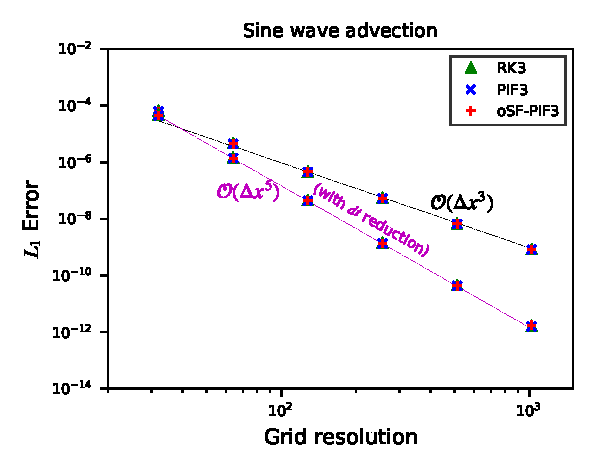
\includegraphics[width=0.85\textwidth]{fig/sine_over_dtReduction}
    \caption{Convergence test for the 1D sine wave advection problem.
        The errors are calculated
        in \( L_{1} \) sense against the initial density profile
        resolved on the computational grids refined
        from 32 to 1024 by a factor of 2.
        All numerical solutions follow the theoretical third-order convergence rate
        (the black-dotted line) when using the timesteps 
        computed from the Courant condition.
        Also plotted are the solutions of using reduced timesteps, which follows the
        fifth-order convergence rate represented in the pink-dotted line.
    }\label{fig:sine_wave}
\end{figure}

The simulation domain is defined on a one-dimensional box of \( [0, 1] \)
with the periodic boundary condition on both ends.
The density profile will propagate one period through the computational domain
and will return to its initial position at \( t = 1 \).
In return, any shape deformation of the density profile
from the initial density profile can be considered as a numerical error
associated with phase errors or numerical diffusions.
The accuracy of the numerical solutions is measured by computing \( L_{1} \) error
between the initial and the final density profiles.
The numerical experiment results from the sine wave advection test
on different number of grid points, \( N_{x} = 32, 64, 128, 256, 512, \) and \( 1024 \)
are depicted in~\cref{fig:sine_wave} for three different temporal methods, Rk3, PIF3, and oSF-PIF3.

There are two types of convergence rates demonstrated in~\cref{fig:sine_wave}.
In the first type, the numerical solutions of three different temporal methods
advanced with timesteps computed from the Courant condition with \( C_{\text{cfl}} = 0.7 \).
Interestingly, the numerical solutions from all three different temporal methods
show a third-order convergence rate, indicating that the leading error term from
third-order temporal methods dominates the spatial error from the fifth-order WENO-JS method.
These results are different from~\cref{fig:vortex_error_saturation},
calculating \( L_{1} \) error from the 2D nonlinear vortex advection case,
where the solution accuracy follows the spatial order at low-resolution regions
until the leading error of the solution is caught up by the temporal error
as computational grids get further refined to higher resolutions.
However, in this test case, the third-order temporal accuracy quickly takes control
throughout the entire range of the grid resolutions tested herein.
This solution behavior strongly supports the importance of
integrating spatially reconstructed solutions with a temporal scheme whose accuracy is
sufficiently high enough to be well comparable to that of the spatial solver.

In the second type of the convergence rate, on the other hand, the timesteps are restricted
in order to match up the lower third-order temporal accuracy with the higher fifth-order spatial accuracy.
Following the usual trick of timestep reduction in~\cite{mignone2010high},
the timestep \( \Delta t_{N} \) is manually adjusted on a grid size of \( N \)
to satisfy the equal rate of change between the spatial and temporal variations.
The restricted timestep is defined by,
\begin{equation}\label{eq:dt_reduction}
    {\Delta t_N} = {\Delta t_0} \Big( \frac{\Delta x_N}{\Delta x_0} \Big)^{\frac{5}{3}},
\end{equation}
where the sub-indices ``0'' and \( N \) refer to the time and grid scales
on a nominal coarse and fine resolution, respectively.
In the current configuration, \( \Delta x_{0} \) is the grid-scale of \( N_{x} = 32 \),
and \( \Delta t_{0} \) is the corresponding timestep subject to the Courant condition with \( C_{\text{cfl}} = 0.7 \).
With the timestep reduction, the overall leading error from the spatial and temporal methods
are matched with the fifth-order spatial accuracy of WENO5,
and the numerical solution of PIF3 and oSF-PIF3 follows the fifth-order convergence rate as expected.
In all test cases for linear advection problems, the oSF-PIF3 solutions behave
almost equally well with the solutions of the original PIF3 and RK3 both quantitatively and qualitatively.



\subsection{Nonlinear isentropic vortex advection}\label{subsec:weno_vortex}

The isentropic vortex advection problem~\cite{shu1998essentially} is one of the most popular benchmark tests
to measure the numerical method's accuracy and performance in the nonlinear case.
Although the problem is fully nonlinear, the exact solution always exists
in the form of its initial condition,
from which an isentropic vortex is advected through periodic boundaries in a 2D computational box.
The accuracy of a numerical method on a nonlinear problem
can be evaluated by comparing the final density profile with the initial condition.

The initial condition consists of a constant background mean flow with \( \rho = 1 \),
\( (u, v) = (1,1) \) and \( p =1 \) on the 2D computaional domain
with periodic boundary conditions.
The isentropic vortex is given by the velocity perturbations \( (\delta u, \delta v) \),
and the temperature perturbation \( \delta T \).
The perturbation terms are designed to set the constant entropy \( S \)
everywhere in the simulation domain, i.e., \( \delta S = 0 \).
The perturbations are given as,
\begin{equation}\label{eq:isentropic_vortex_initial}
    \left( \delta u, \delta v \right) = \frac{\epsilon}{2 \pi} e^{-\half \left( 1 - r^{2} \right)} (-y, x), \quad
    \delta T = - \frac{\left( \gamma - 1 \right) \epsilon^{2}}{8 \gamma \pi^{2}} e^{1 - r^{2}},
\end{equation}
where \( \epsilon = 5 \) is the vortex strength and \( r^{2} = x^{2} + y^{2} \).
The vortex is initially located at the domain center,
and it advects to the diagonal directions, then returns to its original position after one cycle.
The simulation domain size is doubled-up as \( [0, 20] \times [0, 20] \)
compared to the original setup in~\cite{shu1998essentially},
to prevent vortex-vortex couplings near the periodic boundaries
as reported in~\cite{spiegel2015survey}.

\begin{figure}
    \centering
    \begin{subfigure}{70mm}
        \centering
        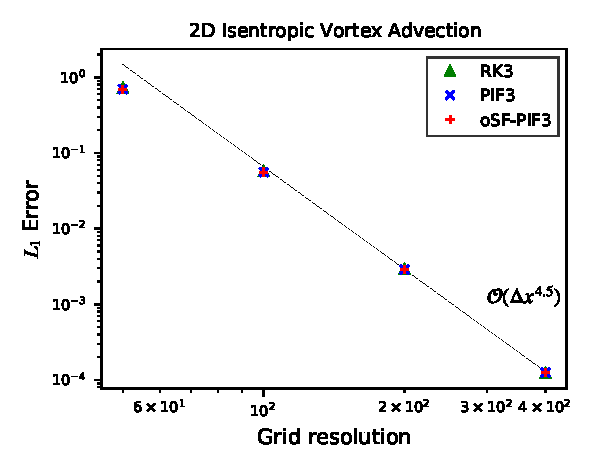
\includegraphics[width=0.95\textwidth]{fig/vortex_third}
    \end{subfigure}
    \begin{subfigure}{70mm}
        \centering
        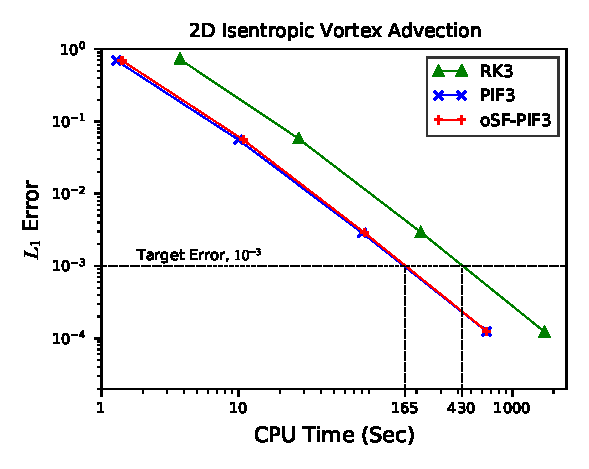
\includegraphics[width=0.95\textwidth]{fig/vortex_time_third}
    \end{subfigure}
    \caption{The \( L_{1} \) errors of the isentropic vortex advection test problem
        solved from third-order temporal schemes combined with WENO5 spatial method.
        The \( L_{1} \) errors
        with respect to the grid resolutions (\textbf{left});
        with respect to the computation time (\textbf{right}).
    }\label{fig:vortex_third}
\end{figure}

\begin{figure}
    \centering
    \begin{subfigure}{70mm}
        \centering
        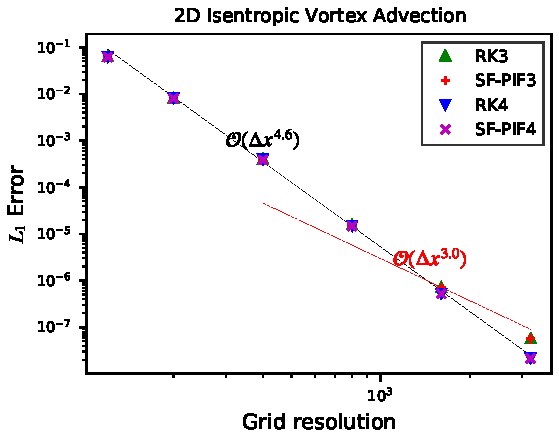
\includegraphics[width=0.95\textwidth]{fig/weno5_vortex_error_fourth}
    \end{subfigure}
    \begin{subfigure}{70mm}
        \centering
        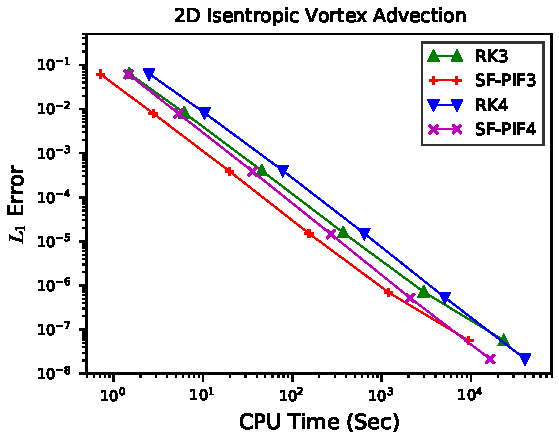
\includegraphics[width=0.95\textwidth]{fig/weno5_vortex_time_fourth}
    \end{subfigure}
    \caption{The \( L_{1} \) errors of the isentropic vortex advection test problem
        solved from third- and fourth-order temporal schemes combined with WENO5 spatial method.
        The \( L_{1} \) errors
        with respect to the grid resolutions (\textbf{left});
        with respect to the computation time (\textbf{right}).
    }\label{fig:vortex_third}
\end{figure}






\subsection{Sod shock tube problem}\label{subsec:sod}


\subsection{Implosion test}\label{subsec:implosion}


\subsection{Shallow water equations}\label{subsec:shallow}



\section{SF-PIF method with WENO-JS}\label{sec:result_wenojs}

\noter{All recursive SF-PIFs}

\subsection{The Shu-Osher problem (rotated \(\ang{45}\))}\label{subsec:weno_shu45}

\subsection{2D Riemann problem: Configuration 3}\label{subsec:weno_2drp_c3}

\subsection{Double Mach reflection}\label{subsec:weno_dmr}



\section{SF-PIF method with GP-WENO}\label{sec:result_gpweno}

\subsection{Hyperparameters}\label{subsec:result_gp_hyper_params}

\subsection{2D Riemann problem: Configuration 3}\label{subsec:gp_2drp_c3}

\noter{what else...}

